%%%%%% Configurando os pacotes e comandos %%%%%%
\documentclass[fontsize=10pt]{article}
\usepackage[margin=0.70in]{geometry}
\usepackage{lipsum,mwe,abstract}
\usepackage[T1]{fontenc} 
\usepackage[brazilian]{babel} 
\usepackage{setspace}
\usepackage{caption}
\usepackage[hidelinks]{hyperref}
\usepackage{multirow}
\usepackage{booktabs}
\usepackage{float}

\usepackage{fancyhdr} % Custom headers and footers
%\pagestyle{fancyplain} % Makes all pages in the document conform to the custom headers and footers
%\fancyhead{} 
%\fancyfoot[C]{\thepage} % Page numbering for right footer
\setlength\parindent{0pt} 
\setstretch{1.5}

\usepackage{xcolor}
% Definindo novas cores
\definecolor{verde}{rgb}{0,0.5,0}
% Configurando layout para mostrar codigos C++
\usepackage{listings}
\lstset{
  language=C,
  basicstyle=\ttfamily\small,
  keywordstyle=\color{purple},
  stringstyle=\color{cyan},
  commentstyle=\color{verde},
  extendedchars=true,
  showspaces=false,
  showstringspaces=false,
  numbers=left,
  numberstyle=\tiny,
  breaklines=true,
  backgroundcolor=\color{blue!10},
  breakautoindent=true,
  captionpos=b,
  xleftmargin=0pt,
}

\usepackage{amsmath,amsfonts,amsthm} % Math packages
\usepackage{wrapfig}
\usepackage{graphicx}
\usepackage{float}
\usepackage{subcaption}
\usepackage{comment}
\usepackage{enumitem}
\usepackage{cuted}
\usepackage{sectsty} % Allows customizing section commands
\allsectionsfont{\normalfont \normalsize \scshape} % Section names in small caps and normal fonts

\renewenvironment{abstract} % Change how the abstract look to remove margins
 {\small
  \begin{center}
  \bfseries \abstractname\vspace{-.5em}\vspace{0pt}
  \end{center}
  \list{}{%
    \setlength{\leftmargin}{0mm}
    \setlength{\rightmargin}{\leftmargin}%
  }
  \item\relax}
 {\endlist}
 
\makeatletter
\renewcommand{\maketitle}{\bgroup\setlength{\parindent}{0pt}% Change how the title looks like
\begin{center}
    \textbf{
      Universidade de São Paulo\\
      Instituto de Ciências Matemáticas e Computação
    }
\end{center}
\begin{center}
  \textbf{\@title}
  \@author\\
  [3pt] 
  \@date
\end{center}\egroup
}
\makeatother
%%% Daqui pra cima é apenas configuração %%%
%%%%%%%%%%%%%%%%%%%%%%%%%%%%%%%%%%%%%%%%%%%%

%%%%%% Definindo seus dados %%%%%%

\title{\Large{Análise de algoritmos de ordenação: \\ [-6pt] Counting Sort, Bucket Sort e Radix Sort} \\ [10pt]} 
\author{Ana Lívia Ruegger Saldanha} 
\date{\today}

%%%%%%%%%%%%%%%%%%%%%%%%%%%%%%%%%%%

%%%%%% Iniciando seu relatório %%%%%% 
\begin{document}
\maketitle


%%%%%%%%%%%%%%%%%%%%%%%%%%%%%%%%%%%%%%%%%%%%%%%%%%%%%%%%%%%
%%%                       RESUMO                        %%%
%%%%%%%%%%%%%%%%%%%%%%%%%%%%%%%%%%%%%%%%%%%%%%%%%%%%%%%%%%%
\begin{abstract}
    %%%%%% Contextualize o seu trabalho. %%%%%%%
    Este relatório apresenta uma análise teórica e experimental acerca da eficiência de três algoritmos de ordenação: counting sort, bucket sort e radix sort. Com base na bibliografia, cada algoritmo é brevemente debatido a partir de seu funcionamento e implementação em linguagem C, identificando-se suas respectivas complexidades assintóticas (notações Big-O e Big-Omega). Essa análise é complementada com os dados obtidos experimentalmente através de medições temporais feitas também em linguagem C. Na parte experimental, esses três algoritmos também são comparados com outros três: quick sort, heap sort e merge sort.
    
\end{abstract}

\rule{\linewidth}{0.5pt}

%%%%%%%%%%%%%%%%%%%%%%%%%%%%%%%%%%%%%%%%%%%%%%%%%%%%%%%%%%%
%%%                    1 INTRODUÇÃO                     %%%
%%%%%%%%%%%%%%%%%%%%%%%%%%%%%%%%%%%%%%%%%%%%%%%%%%%%%%%%%%%
\section{Introdução}
%%%%%% Faça a introdução do seu relatório. O que será feito? %%%%%%
    
    \quad O problema da ordenação apresentado por Cormen no primeiro capítulo de \textit{Algoritmos: teoria e prática} \cite{cormen} é frequentemente estudado como introdução aos conceitos de algoritmos e eficiência. Pode ser definido formalmente da seguinte maneira:
    
    \begin{itemize}
        \item \textbf{Entrada:} Uma sequência de $n$ números $<a_1, a_2, ..., a_n>$.
        \item \textbf{Saída:} Uma permutação (reordenação) $<a_1', a_2', ..., a_n'>$ da sequência de entrada, tal que $a_1' \leq a_2' \leq ... \leq a_n'$.
    \end{itemize}
    
    \quad Para solucioná-lo, podemos utilizar diversos algoritmos, mas, mesmo que todos sejam corretos e resolvam o problema dado, esses algoritmos podem ser muito diferentes em termos de eficiência. Neste relatório, temos por objetivo debater essa questão através da análise e comparação de seis algoritmos de ordenação: counting sort (ordenação por contagem), bucket sort (ordenação por balde), radix sort (ordenação digital), merge sort (ordenação por intercalação), quick sort e heap sort, com enfoque nos três primeiros, sobre os quais apresentaremos uma análise teórica mais aprofundada, visto que os outros já foram estudados em relatórios anteriores\cite{relatorio1}\cite{relatorio2}. 
    
    \quad Primeiramente, buscamos contextualizar esses três algoritmos (counting, bucket e radix sort), apresentando seu funcionamento básico e implementações em linguagem C, assim como as funções obtidas através da contagem de operações de cada algoritmo e respectivas análises utilizando o conjunto de notações assintóticas Big-O ($\mathcal{O}$) e Big-Omega ($\Omega$).
    
    \quad Em seguida, apresentamos os resultados de um experimentos realizados com os seis algoritmos através de medições temporais. Os experimentos têm por objetivo comprovar as discussões levantadas anteriormente para que possamos, por fim, realizar uma análise abrangente desses algoritmos em diferentes cenários.


%%%%%%%%%%%%%%%%%%%%%%%%%%%%%%%%%%%%%%%%%%%%%%%%%%%%%%%%%%%
%%%           2 METODOLOGIA E DESENVOLVIMENTO           %%%
%%%%%%%%%%%%%%%%%%%%%%%%%%%%%%%%%%%%%%%%%%%%%%%%%%%%%%%%%%%
\section{Metodologia e desenvolvimento}
%%%%%% Explique a metodologia utilizada e o desenvolvimento do projeto. Como você obteve seus dados? Coloque seus códigos e embasamentos teóricos aqui se necessário. %%%%%%

\quad Nos relatórios anteriores, foram estudados algoritmos de ordenação baseados em comparação, isto é, que realizam a ordenação de um conjunto comparando seus valores entre si. Para estes algoritmos, o desempenho alcançado não consegue vencer o limite inferior $n \cdot log(n)$ no pior caso.\footnote{Esta afirmação é provada por Cormen et al. na seção 8.1, \textit{Limites inferiores para ordenação}, do livro \textit{Algoritmos: teoria e prática}\cite{cormen}, levando em consideração que as ordenações por comparação funcionam como \textbf{árvores de decisão}.} Neste relatório, nos focaremos em algoritmos de ordenação linear — \textit{counting}, \textit{bucket} e \textit{radix sort} —, que são capazes de vencer essa barreira $n \cdot log(n)$, porém necessitam de memória auxiliar que depende não apenas do tamanho $n$ do conjunto a ser ordenado, mas também da diferença entre os valores da maior e da menor chave presentes nesse conjunto (chamaremos essa amplitude de $k$).

\quad Para estabelecer um padrão, estudaremos os três algoritmos em suas versões que trabalham com registros\footnote{As implementações utilizadas no experimento e reproduzidas neste relatório estão de acordo com o material apresentado em aula pelo professor Fernando Pereira dos Santos\cite{lab}. Já as análises apresentadas foram baseadas tanto nas aulas quanto na bibliografia, especialmente no livro \textit{Algoritmos: teoria e prática} (Cormen et al.)\cite{cormen}.}, adotando o tipo definido abaixo (em linguagem C):

\begin{lstlisting}
typedef struct registro
{
    int chave;
    // Outros atributos
    // (...)
}   registro_t;
\end{lstlisting}

\quad Adiante, discutiremos mais a fundo o Counting Sort, o Bucket Sort e o Radix Sort, trazendo também um resumo do que já foi apresentado sobre o Quick Sort, o Heap Sort e o Merge Sort \cite{relatorio1}\cite{relatorio2}.

%%%%% 2.1 COUNTING SORT %%%%%
\subsection{Counting Sort}

\quad O \textit{counting sort} é um algoritmo que ordena um conjunto a partir de chaves inteiras. Sua heurística é baseada na contagem dos elementos que apresentam dada chave, utilizando esse mesmo valor chave para indexar um vetor de tamanho $k$ que armazena a contagem em si (por isso, é preciso trabalhar com inteiros); essa contagem, por sua vez, é utilizada para determinar o índice final de cada elemento no conjunto ordenado.

\quad Pelo processo descrito acima, podemos notar que o \textit{counting sort} necessita, pelo menos, de um vetor auxiliar de tamanho $k$; sua implementação tradicional, portanto, pertence a $\mathcal{O}(k)$ quanto ao uso de memória. Porém, como poderemos observar adiante, na implementação que utilizamos — que trabalha com registros — precisamos de uma cópia do vetor original; neste caso, o \textit{counting sort} pertence a $\mathcal{O}(n + k)$

\quad A seguir, apresentamos a implementação do \textit{counting sort} com registros, em linguagem C.

\begin{lstlisting}
void counting_sort(registro_t *vetor, int tamanho)
{
    registro_t *copia = (registro_t *)malloc(tamanho * sizeof(registro_t));

    int max, min;
    max = min = vetor[0].chave;
    
    for (int i = 0; i < tamanho; i++)
    {
        if (vetor[i].chave > max)
            max = vetor[i].chave;
        if (vetor[i].chave < min)
            min = vetor[i].chave;
        copia[i] = vetor[i];
    }

    int k = max - min + 1;
    int *contagem = (int *)calloc(k, sizeof(int));

    for (int i = 0; i < tamanho; i++)
    {
        int posicao_chave = vetor[i].chave - min;
        contagem[posicao_chave]++;
    }

    int total = 0;
    for (int i = 0; i < k; i++)
    {
        int contagem_anterior = contagem[i];
        contagem[i] = total;
        total = total + contagem_anterior;
    }

    for (int i = 0; i < tamanho; i++)
    {
        int posicao_ordenada = contagem[copia[i].chave - min];
        vetor[posicao_ordenada] = copia[i];
        contagem[copia[i].chave - min]++;
    }

    free(contagem);
    free(copia);
}
\end{lstlisting}

\quad Pela lógica mostrada no código acima, podemos observar que, quanto à complexidade de tempo, o \textit{counting sort} também é diretamente influenciado pelos valores de $k$ e $n$. Dessa forma, para realizar a análise assintótica, precisamos observar quantas vezes o algoritmo percorre cada vetor de tamanho $n$ ou $k$; esse processo pode ser facilmente observado nos \textbf{laços} presentes no código:

\begin{itemize}
    \item O primeiro laço, iniciado na linha 8, percorre o vetor original de tamanho $n$ para realizar uma cópia dos dados e também buscar as chaves máxima e mínima; tem, portanto, complexidade de tempo $\mathcal{O}(n)$.
    
    \item Um segundo laço está presente na inicialização do vetor de contagem de tamanho $k$, sendo implícito na função \texttt{calloc} (linha 18); pertence a $\mathcal{O}(k)$.
    
    \item O terceiro laço (linha 20) percorre o conjunto inicial de tamanho $n$ realizando a contagem das chaves; pertence a $\mathcal{O}(n)$.
    
    \item O quarto laço (linha 27) realiza a contagem acumulada das chaves, ou seja, determina as posições finais no conjunto ordenado; pertence a $\mathcal{O}(k)$.
    
    \item Finalmente, o último laço (linha 34) realiza o posicionamento final dos elementos no conjunto ordenado; pertence a $\mathcal{O}(n)$.
\end{itemize}

\quad O \textit{counting sort}, dessa forma, percorre três vezes um vetor de tamanho $n$ e duas vezes um vetor de tamanho $k$, resultando na complexidade de tempo $\mathcal{O}(n + k)$. Podemos observar, também, que seu funcionamento dependerá sempre dos valores de $n$ e $k$, de forma que ele jamais será capaz de ultrapassar o limite inferior de $n + k$; pertence, portanto, a $\Omega(n + k)$.

\quad Outra característica do \textit{counting sort} que devemos destacar é que este se trata de um algoritmo \textbf{estável}, ou seja, que preserva, no conjunto final, a ordem inicial dos elementos que possuem a mesma chave. Como veremos adiante, este é um fator essencial quando utilizamos a ordenação por contagem como sub-rotina do \textit{radix sort}.

%%%%% 2.2 BUCKET SORT %%%%%
\subsection{Bucket Sort}

\quad O \textit{bucketsort}, ou ordenação por balde, funciona a partir da distribuição dos elementos de um conjunto em listas encadeadas chamadas de baldes. Estas listas, então, podem ser ordenadas por outro algoritmo de ordenação, ou recursivamente pelo próprio \textit{bucketsort}; por fim, basta que, percorrendo balde por balde, os elementos sejam reposicionados no conjunto final ordenado. A implementação aqui estudada, no entanto, possui uma particularidade: cada lista, ou balde, está associada a uma chave específica\footnote{Este tipo específico de \textit{bucketsort} também é conhecido como \textit{pigeonhole sort}.} (portanto, não há uma sub-rotina de ordenação das listas).

\quad Além da \textit{struct} registro reproduziada anteriormente, no \textit{bucketsort} utilizamos as seguintes declarações de nó e lista encadeada (balde):

\begin{lstlisting}
typedef struct no
{
    registro_t elem;
    struct no *prox;
}   no_t;

typedef struct balde
{
    no_t *inicio;
    no_t *fim;
}   balde_t;
\end{lstlisting}

\quad Declaradas as \textit{structs} acima, a implementação do \textit{bucketsort} em linguagem C é dada da seguinte forma:

\begin{lstlisting}
void bucket_sort(registro_t *vetor, int tamanho)
{
    int max, min;
    max = min = vetor[0].chave;
    for (int i = 1; i < tamanho; i++)
    {
        if (vetor[i].chave > max)
            max = vetor[i].chave;
        if (vetor[i].chave < min)
            min = vetor[i].chave;
    }

    int k = max - min + 1;
    balde_t *baldes = (balde_t *)calloc(k, sizeof(balde_t));

    for (int i = 0; i < tamanho; i++)
    {
        int posicao_chave = vetor[i].chave - min;

        no_t *novo = malloc(sizeof(no_t));
        novo->elem = vetor[i];
        novo->prox = NULL;

        if (baldes[posicao_chave].inicio == NULL)
            baldes[posicao_chave].inicio = novo;
        else
            (baldes[posicao_chave].fim)->prox = novo;
        baldes[posicao_chave].fim = novo;
    }

    int j = 0;
    for (int i = 0; i < k; i++)
    {
        no_t *posicao;
        posicao = baldes[i].inicio;
        while (posicao != NULL)
        {
            vetor[j] = posicao->elem;
            j++;

            no_t *deletar = posicao;
            posicao = posicao->prox;
            baldes[i].inicio = posicao;
            free(deletar);
        }
    }

    free(baldes);
}
\end{lstlisting}

\quad Nessa implementação em específico, a complexidade de tempo do \textit{bucketsort} é similar à do \textit{counting sort} e pode ser compreendida observando os laços presentes no código. O algoritmo percorre duas vezes um vetor de tamanho $n$: para verificar os valores máximo e mínimo dentre as chaves (linha 5) e para preencher os baldes (linha 16); por fim, para reposicionar os elementos no vetor original, retirando-os dos baldes, o algoritmo também percorre $n$ nós no total (a partir da linha 32). Já o vetor de baldes, de tamanho $k$, é percorrido duas vezes: quando é inicializado pela função \texttt{calloc} (linha 14) e no processo de reposicionamento dos elementos no conjunto ordenado (a partir da linha 32).

\quad A partir dessa análise, podemos afirmar que, assim como o \textit{counting sort}, o \textit{bucketsort} pertence a $\mathcal{O}(n + k)$, e sempre será dependente desses dois valores; dessa forma, esse método também não poderá ultrapassar o limite inferior de $n + k$ — ou seja, o \textit{bucketsort} pertence à $\Omega(n + k)$.

\quad No entanto, não podemos esperar que, na prática, o tempo de ordenação do \textit{bucketsort} seja o mesmo que o do \textit{counting sort}, visto que, ao trabalhar com listas ligadas, esse algoritmo realiza uma quantidade maior de operações (por exemplo, a alocação e a desalocação da memória ocupada pelos nós das listas). Além disso, para uma aplicação vantajosa do \textit{bucketsort}, espera-se que o conjunto de entrada seja uniformemente distribuído, de forma que não tenhamos muitos elementos em um mesmo balde;\footnote{Segundo Cormen et al., na seção 8.4 de \textit{Algoritmos: teoria e prática}\cite{cormen}.} quando isso ocorre, o desempenho desse algoritmo é prejudicado.

\quad O \textit{bucketsort} é um algoritmo \textbf{estável} e também pode ser utilizado como sub-rotina na ordenação digital (\textit{radix sort}).

%%%%% 2.3 RADIX SORT %%%%%
\subsection{Radix Sort}

\quad Como já foi adiantado, o \textit{radix sort} utiliza um dos algoritmos acima como sub-rotina. Também se trata de um método de ordenação linear que necessita de memória auxiliar, mas sua implementação é capaz minimizar a complexidade de tempo e de memória em cenários com $k$ elevado.

\quad A heurística do \textit{radix sort} é baseada na ordenação pelos \textbf{dígitos} das chaves, do menos significativo para o mais significativo; ou seja, um processo de ordenação estável — seja ele o \textit{counting sort} ou o \textit{bucketsort} — será executado uma quantidade $d$ de vezes (uma vez por dígito), resultando, ao fim do processo, na ordenação completa do conjunto. O que chamamos de dígito será definido de acordo com uma base $b$, um valor previamente fixado que, a cada execução da sub-rotina, ocupará o lugar que no \textit{bucket} e no \textit{counting sort} era ocupado por $k$, definindo o tamanho do vetor de contagem.

\quad Aqui, abordaremos uma implementação do \textit{radix sort} que utiliza o \textit{counting sort} como sub-rotina e adota a base $b = 256$ (1 byte); essa implementação, em linguagem C, é reproduzida abaixo:

\begin{lstlisting}
void radix_sort(registro_t *vetor, int tamanho)
{
    int contagem[256] = {0};
    int acumulada[256];
    
    registro_t *copia = (registro_t *)malloc(tamanho * sizeof(registro_t));

    int i, shift;
    for (shift = 0; shift <= 24; shift += 8) 
    {
        for (i = 0; i < tamanho; i++)
        {
            short k = (vetor[i].chave >> shift) & 255;
            contagem[k]++;
            copia[i] = vetor[i];
        }

        acumulada[0] = 0;
        for (i = 1; i < 256; i++)
        {
            acumulada[i] = acumulada[i - 1] + contagem[i - 1];
            contagem[i - 1] = 0;
        }

        for (i = 0; i < tamanho; i++)
        {
            short k = (copia[i].chave >> shift) & 255;
            vetor[acumulada[k]] = copia[i];
            acumulada[k]++;
        }
    }

    free(copia);
}
\end{lstlisting}

\quad Como pode ser observado no código acima, o laço iniciado na linha 9, utilizando de operações de \textit{bit shift}, é responsável por executar o \textit{counting sort} uma vez para cada dígito. Como sabemos que a ordenação por contagem é $\mathcal{O}(n + k)$, poderíamos afirmar que o \textit{radix sort} pertence a $\mathcal{O}(d \cdot (n + k))$; mas, nesse caso, sendo $k$ o valor previamente fixado na base $b$, concluímos que o \textit{radix sort} pertence, na verdade, a $\mathcal{O}(d \cdot (n + b))$. Por outro lado, o algoritmo também não será capaz de vencer o limite inferior de $(d \cdot (n + b))$, sendo, assim, $\Omega((d \cdot (n + b))$.

\quad Para a implementação estudada, sabendo que $b = 256$ e $d = 4$ (pois todas as chaves são inteiros de 4 bytes), temos que este algoritmo é $\mathcal{O}(4 \cdot (n + 256))$. Notemos ainda que, como a base fixa o tamanho do vetor de contagem, o uso de memória no \textit{radix sort} também é controlado (e pode ser manipulado) pelo valor de $b$. Quanto ao uso de memória, portanto, o \textit{radix sort} pertence a $\mathcal{O}(n + b)$.

%%%%% 2.4 COMPARAÇÃO %%%%%
\subsection{Comparação com Quick Sort, Heap Sort e Merge Sort}

\quad Para fins de comparação, a Tabela 1 apresenta as informações essenciais acerca da complexidade do \textit{quick}, do \textit{heap} e do \textit{mergesort}, como demonstrado nos relatórios anteriores\cite{relatorio1}\cite{relatorio2}.

\begin{table}[ht]
\centering
\begin{tabular}{@{}c|c|c|c|c|c@{}}
Algoritmo  & $\mathcal{O}$          & $\Omega$          & Memória auxiliar & Melhor caso    & Pior caso                            \\ \midrule
Quick Sort & $\mathcal{O}(n^2)$     & $\Omega(n\ logn)$ & $\mathcal{O}(1)$ & Pivô no centro & Pivô na extremidade (vetor ordenado) \\
Heap sort  & $\mathcal{O}(n\ logn)$ & $\Omega(n\ logn)$ & $\mathcal{O}(1)$ & -              & -                                    \\
Merge Sort & $\mathcal{O}(n\ logn)$ & $\Omega(n\ logn)$ & $\mathcal{O}(n)$ & -              & -                          
\end{tabular}
\caption{Resumo acerca das complexidades de tempo e espaço dos algoritmos de ordenação Quick Sort, Heap Sort e Merge Sort.}
\label{Tabela 1}
\end{table}

%%%%%%%%%%%%%%%%%%%%%%%%%%%%%%%%%%%%%%%%%%%%%%%%%%%%%%%%%%%
%%%                    3 RESULTADOS                     %%%
%%%%%%%%%%%%%%%%%%%%%%%%%%%%%%%%%%%%%%%%%%%%%%%%%%%%%%%%%%%
\section{Resultados}
    %%%%%% Mostre os resultados obtidos através dos cálculos. Utilize imagens se necessário. %%%%%%

\quad A seguir, apresentamos os resultados de três conjuntos de testes, realizados a fim de estudar, na prática, a eficiência dos algoritmos apresentados na seção anterior deste relatório.

%%%%% 3.1 VETORES GERADOS ALEATORIAMENTE %%%%%    
\subsection{Vetores gerados aleatoriamente}

\quad O primeiro experimento realizado teve como objetivo analisar o desempenho dos algoritmos \textit{counting}, \textit{bucket} e \textit{radix sort} com vetores de entrada cada vez maiores. Destacamos algumas escolhas que fizemos na implementação do experimento:

\begin{itemize}
    \item Executamos três testes com vetores de registros cujos valores das chaves foram gerados aleatoriamente, cada um adotando uma amplitude $k$ diferente: valores entre 0 e $n$, entre 0 e $5n$, e entre 0 e $10n$, sendo $n$ o tamanho da entrada.
    
    \item Para cada tamanho de vetor, realizamos 10 iterações/medições; os valores apresentados nos gráficos a seguir referem-se à média do tempo de execução nessas 10 iterações.
    
    \item Cada teste dos algoritmos foi realizado em uma única execução do programa, com exatamente os mesmos vetores, gerando um arquivo .csv para cada algoritmo. Os dados contidos nesses arquivos foram utilizados para plotar o gráficos reproduzidos a seguir.
\end{itemize}

\quad Como era esperado, por conta do uso de listas ligadas e consequente maior número de operações, o \textit{bucketsort} mostrou-se, nos três testes, o mais lento dentre os algoritmos de ordenação lineares.

\quad Também como previsto, a diferença de eficiência entre o \textit{counting sort} e o \textit{radix sort} é alterada conforme aumentamos a amplitude de valores $k$. No teste com valores entre 0 e $n$, apresentado no gráfico da Figura 1, o \textit{counting sort} mostrou-se mais rápido que o \textit{radix}; com valores entre 0 e $5n$, os dois algoritmos apresentaram desempenho muito similar (Figura 2); finalmente, com valores entre 0 e $10n$, o \textit{radix sort} mostrou-se o mais eficiente dos três algoritmos (Figura 3).

\begin{figure}[]
\begin{center}
    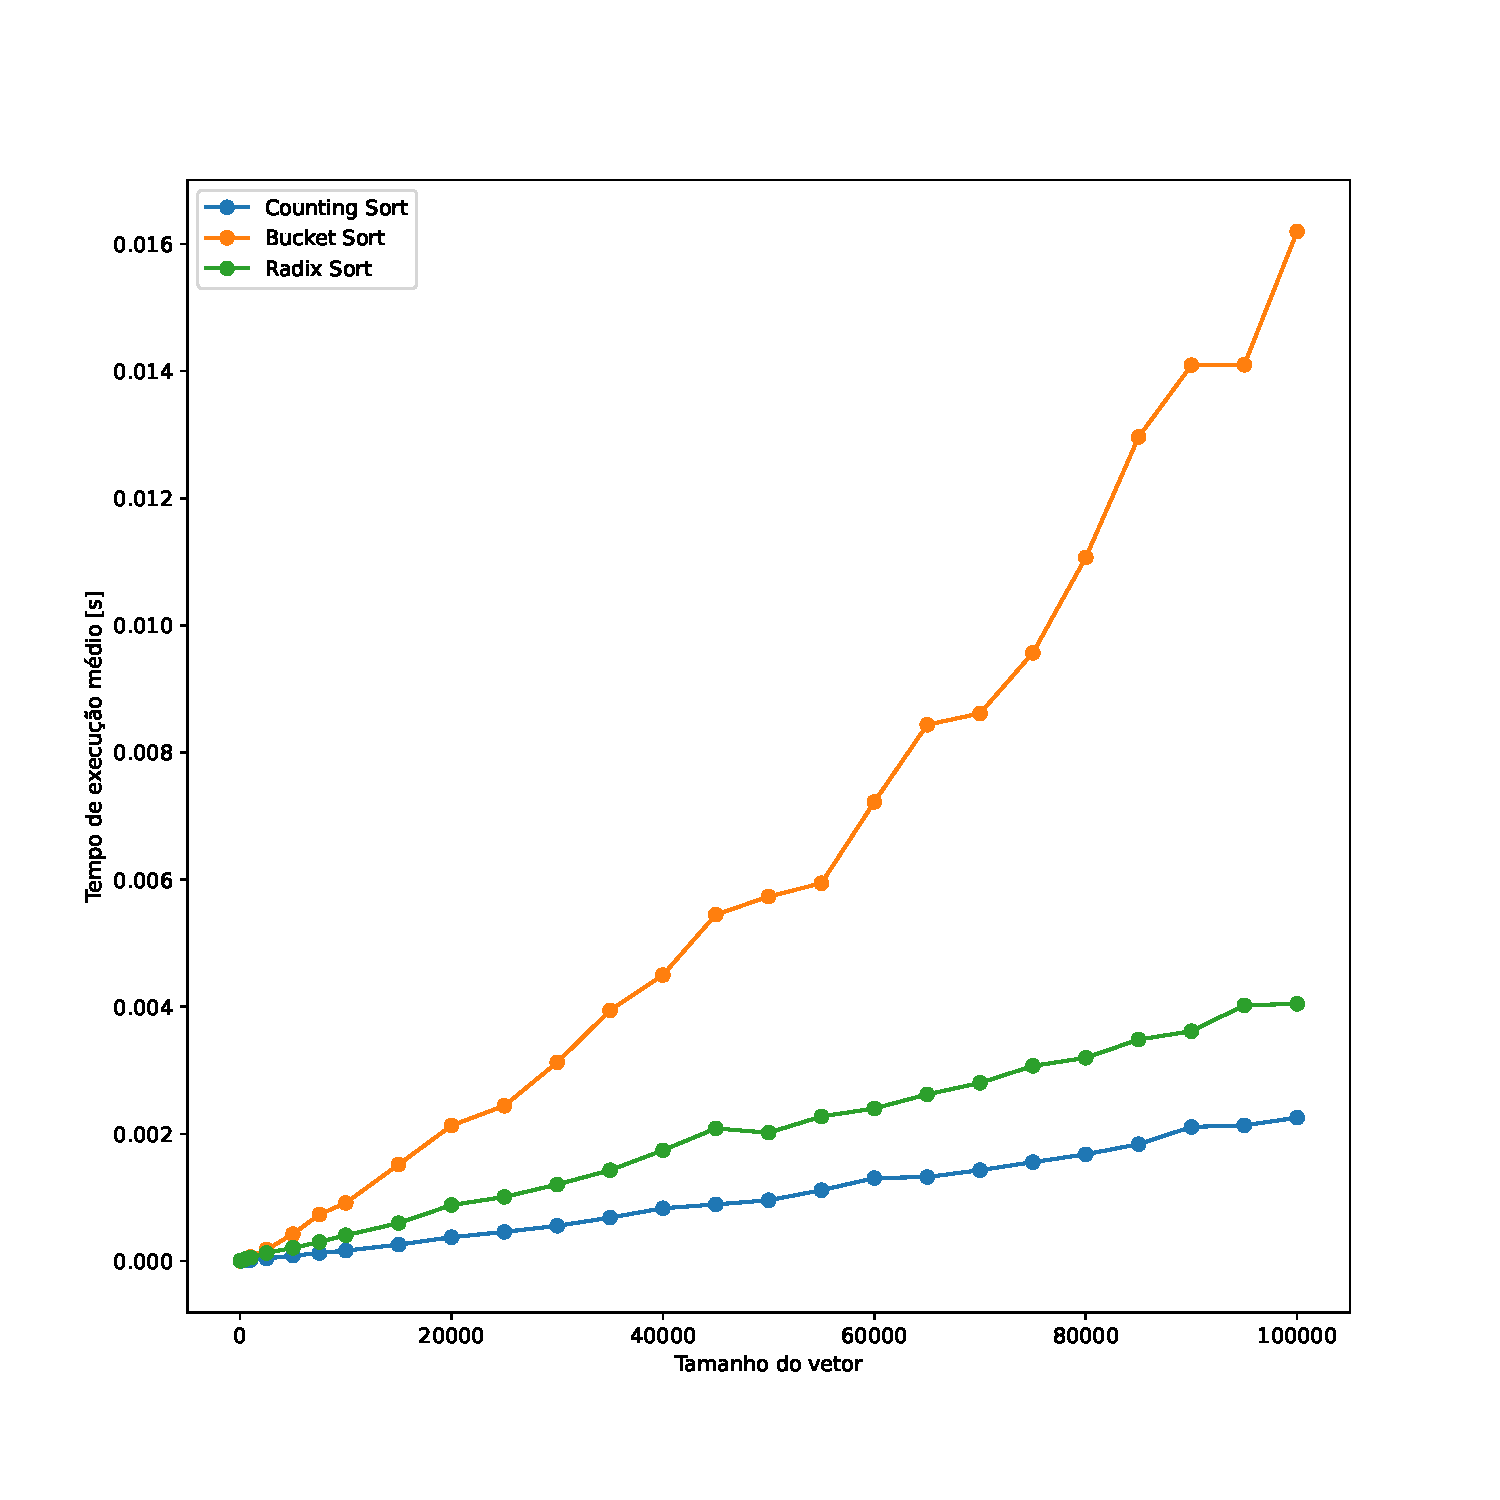
\includegraphics[scale=0.4]{imagens/0302.pdf}
    \caption{Resultado das medições temporais para cada algoritmo, ordenando com chaves de valores entre 0 e $n$; a média de tempo de execução foi tirada a partir de 10 iterações para cada tamanho de vetor.}
    \label{Figura 1}
\end{center}
\end{figure}

\begin{figure}[]
\begin{center}
    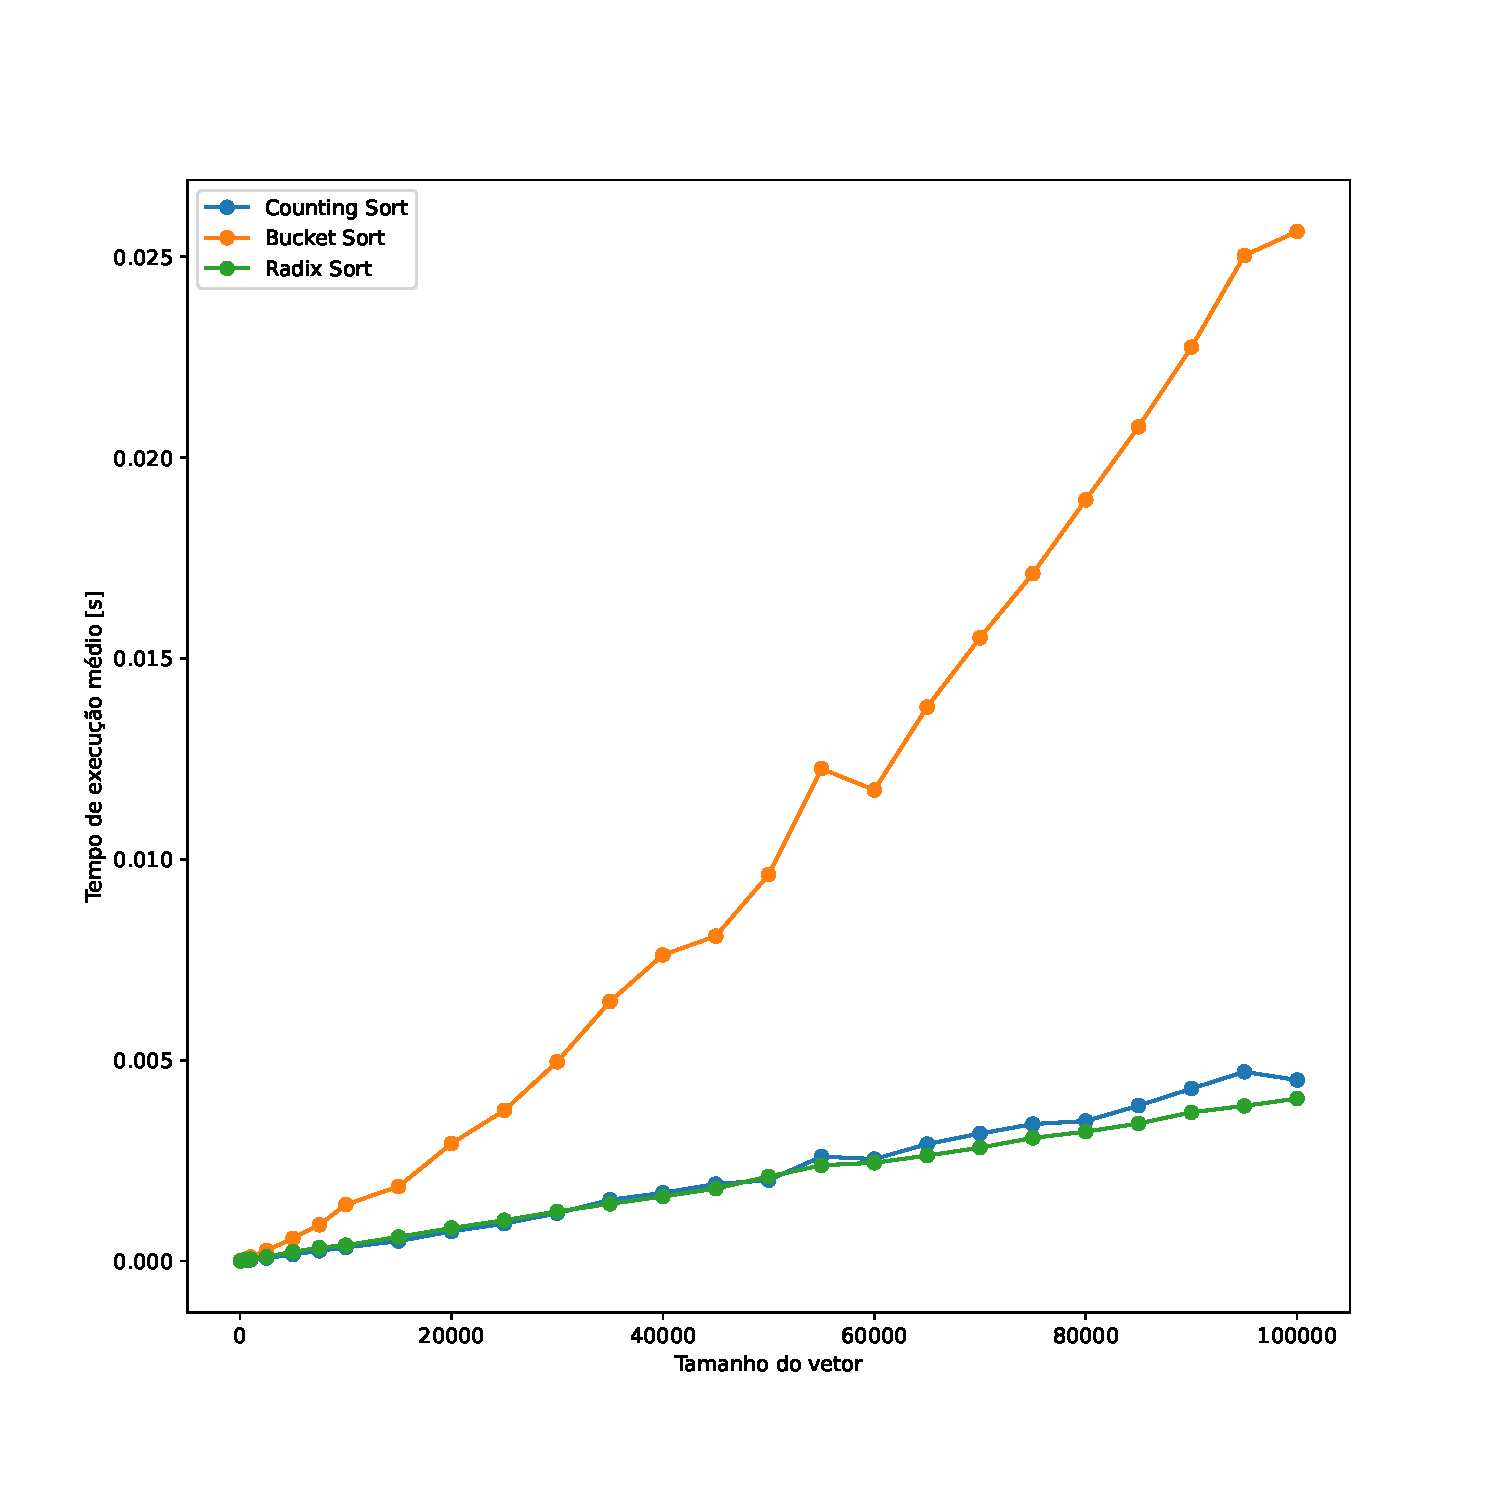
\includegraphics[scale=0.4]{imagens/0502.pdf}
    \caption{Resultado das medições temporais para cada algoritmo, ordenando com chaves de valores entre 0 e $5n$; a média de tempo de execução foi tirada a partir de 10 iterações para cada tamanho de vetor.}
    \label{Figura 2}
\end{center}
\end{figure}

\begin{figure}[H]
\begin{center}
    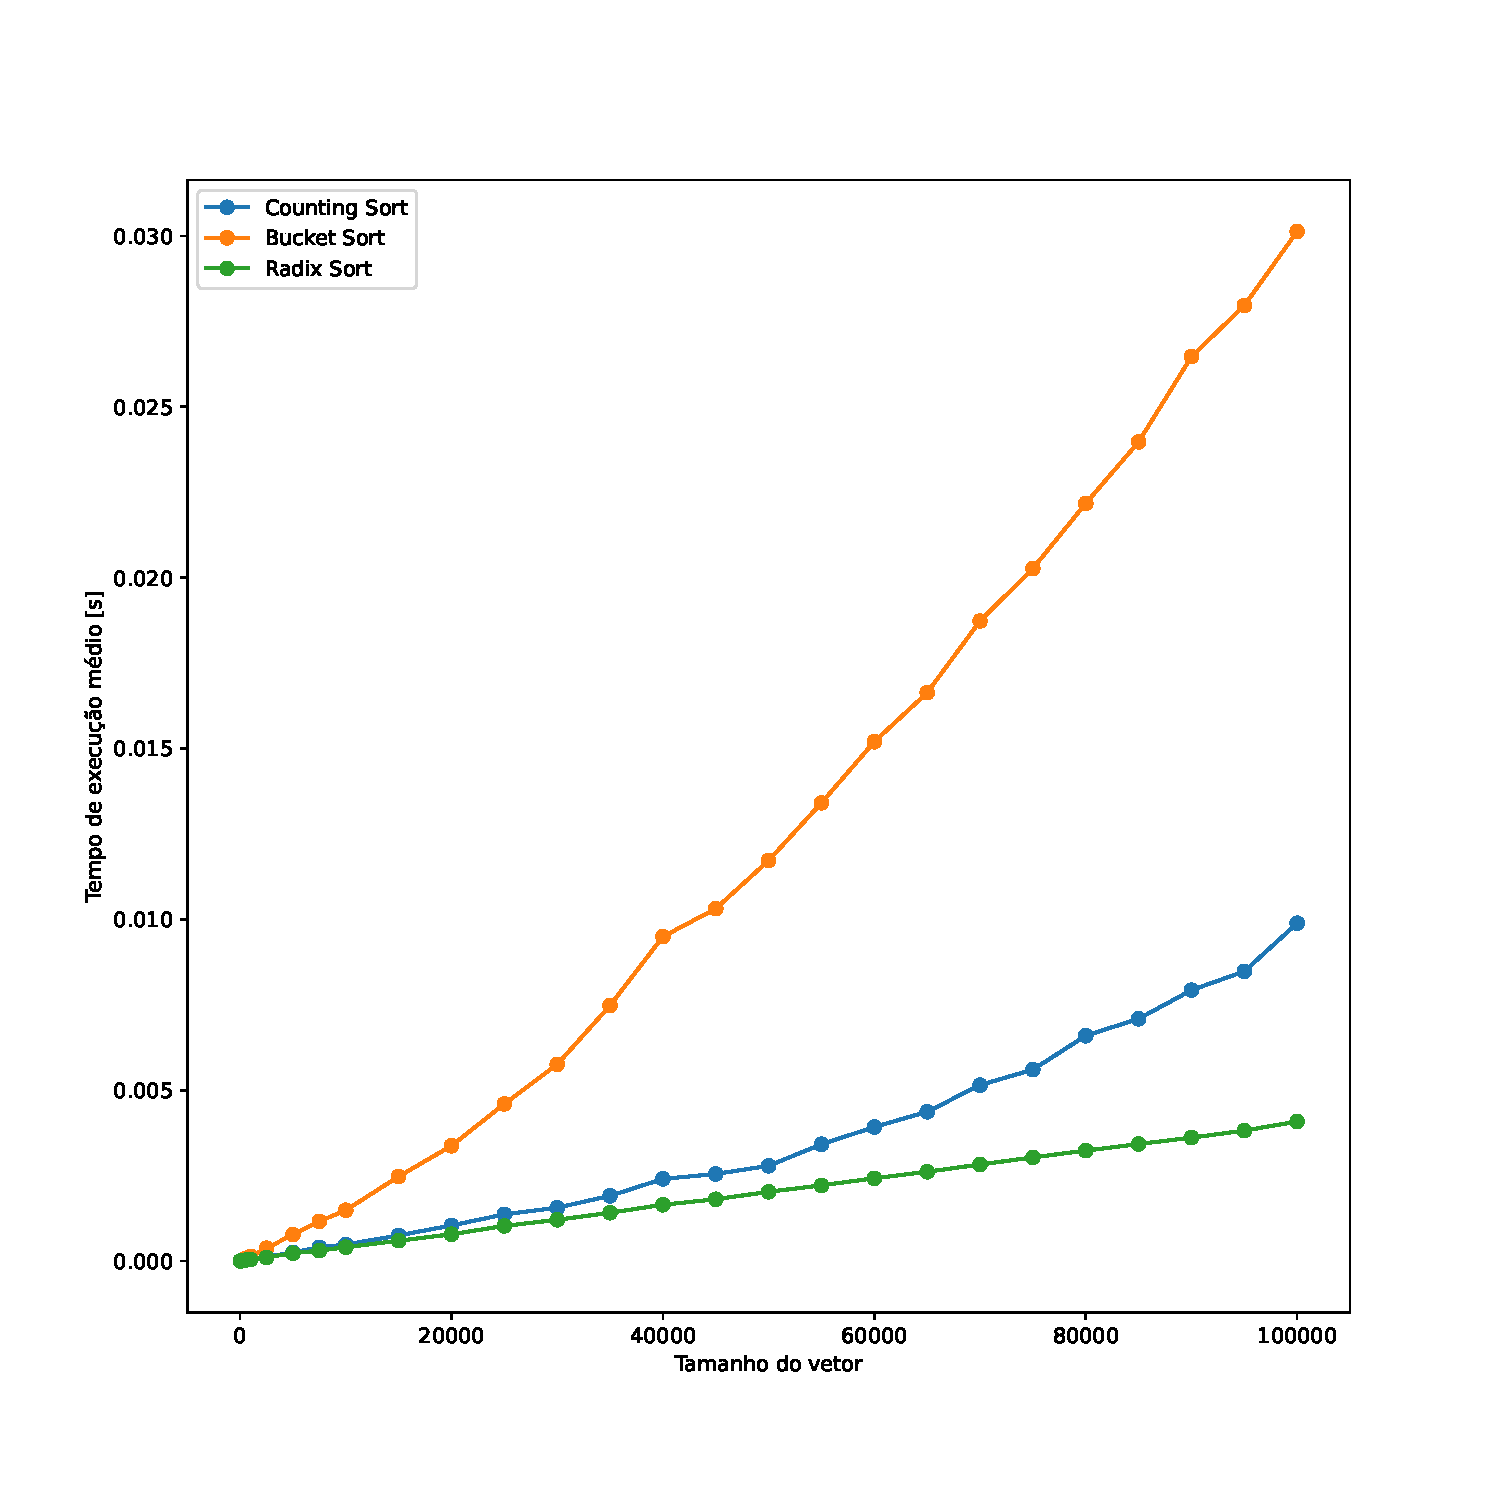
\includegraphics[scale=0.4]{imagens/0602.pdf}
    \caption{Resultado das medições temporais para cada algoritmo, ordenando com chaves de valores entre 0 e $10n$; a média de tempo de execução foi tirada a partir de 10 iterações para cada tamanho de vetor.}
    \label{Figura 3}
\end{center}
\end{figure}

%%%%% 3.2 MELHOR E PIOR CASO %%%%%
\subsection{Melhor e pior caso}

\quad Mantendo o padrão dos experimentos apresentados nos relatórios anteriores\cite{relatorio1}\cite{relatorio2}, realizamos testes com vetores de mesmo tamanho ($n = 1000$), porém de diferentes tipos: gerados aleatoriamente, ordenados e inversamente ordenados.

\begin{table}[ht]
\centering
\begin{tabular}{@{}c|ccc@{}}
Tipo de vetor         & \multicolumn{3}{c}{Tempo de execução médio {[}s{]}} \\
(tamanho $n = 100$)   & \textbf{Counting Sort} & \textbf{Bucket Sort} & \textbf{Radix Sort} \\ \midrule
Gerado aleatoriamente & 0.000019               & 0.000065             & 0.000057            \\
Ordenado              & 0.000020               & 0.000054             & 0.000055            \\
Inversamente ordenado & 0.000019               & 0.000054             & 0.000053         
\end{tabular}
\caption{Resultado das medições temporais para ordenação de diferentes tipos de vetor, todos com o mesmo tamanho; a média de tempo de execução foi tirada a partir de 10 iterações para cada tipo de vetor.}
\label{Tabela 3}
\end{table}

\quad Os resultados mostrados na Tabela 2 confirmam que, de fato, como estes não se tratam de algoritmos baseados em comparação, a ordenação prévia dos elementos do conjunto não altera sua eficiência. No entanto, podemos notar que o \textit{bucketsort} apresentou um desempenho melhor para os vetores ordenados; essa diferença era esperada e não se deve à ordenação em si, mas ao fato de que, nesses vetores, as chaves foram distribuídas uniformemente.

\quad Como visto na seção 2 deste relatório, os algoritmos de ordenação lineares tem seu desempenho diretamente afetado pela amplitude de valores $k$ apresentada nas chaves. Dessa forma, para analisar o que chamamos de \textbf{pior caso} e \textbf{melhor caso}, devemos observar o comportamento de cada um desses algoritmos diante da variação de $k$. Utilizaremos, para tal, os dados do experimento já descrito no item 3.1 — mas, desta vez, apresentados através de gráficos que comparam o desempenho de um mesmo algoritmo nos três cenários diferentes (Figuras 4, 5 e 6).

\begin{figure}[]
\begin{center}
    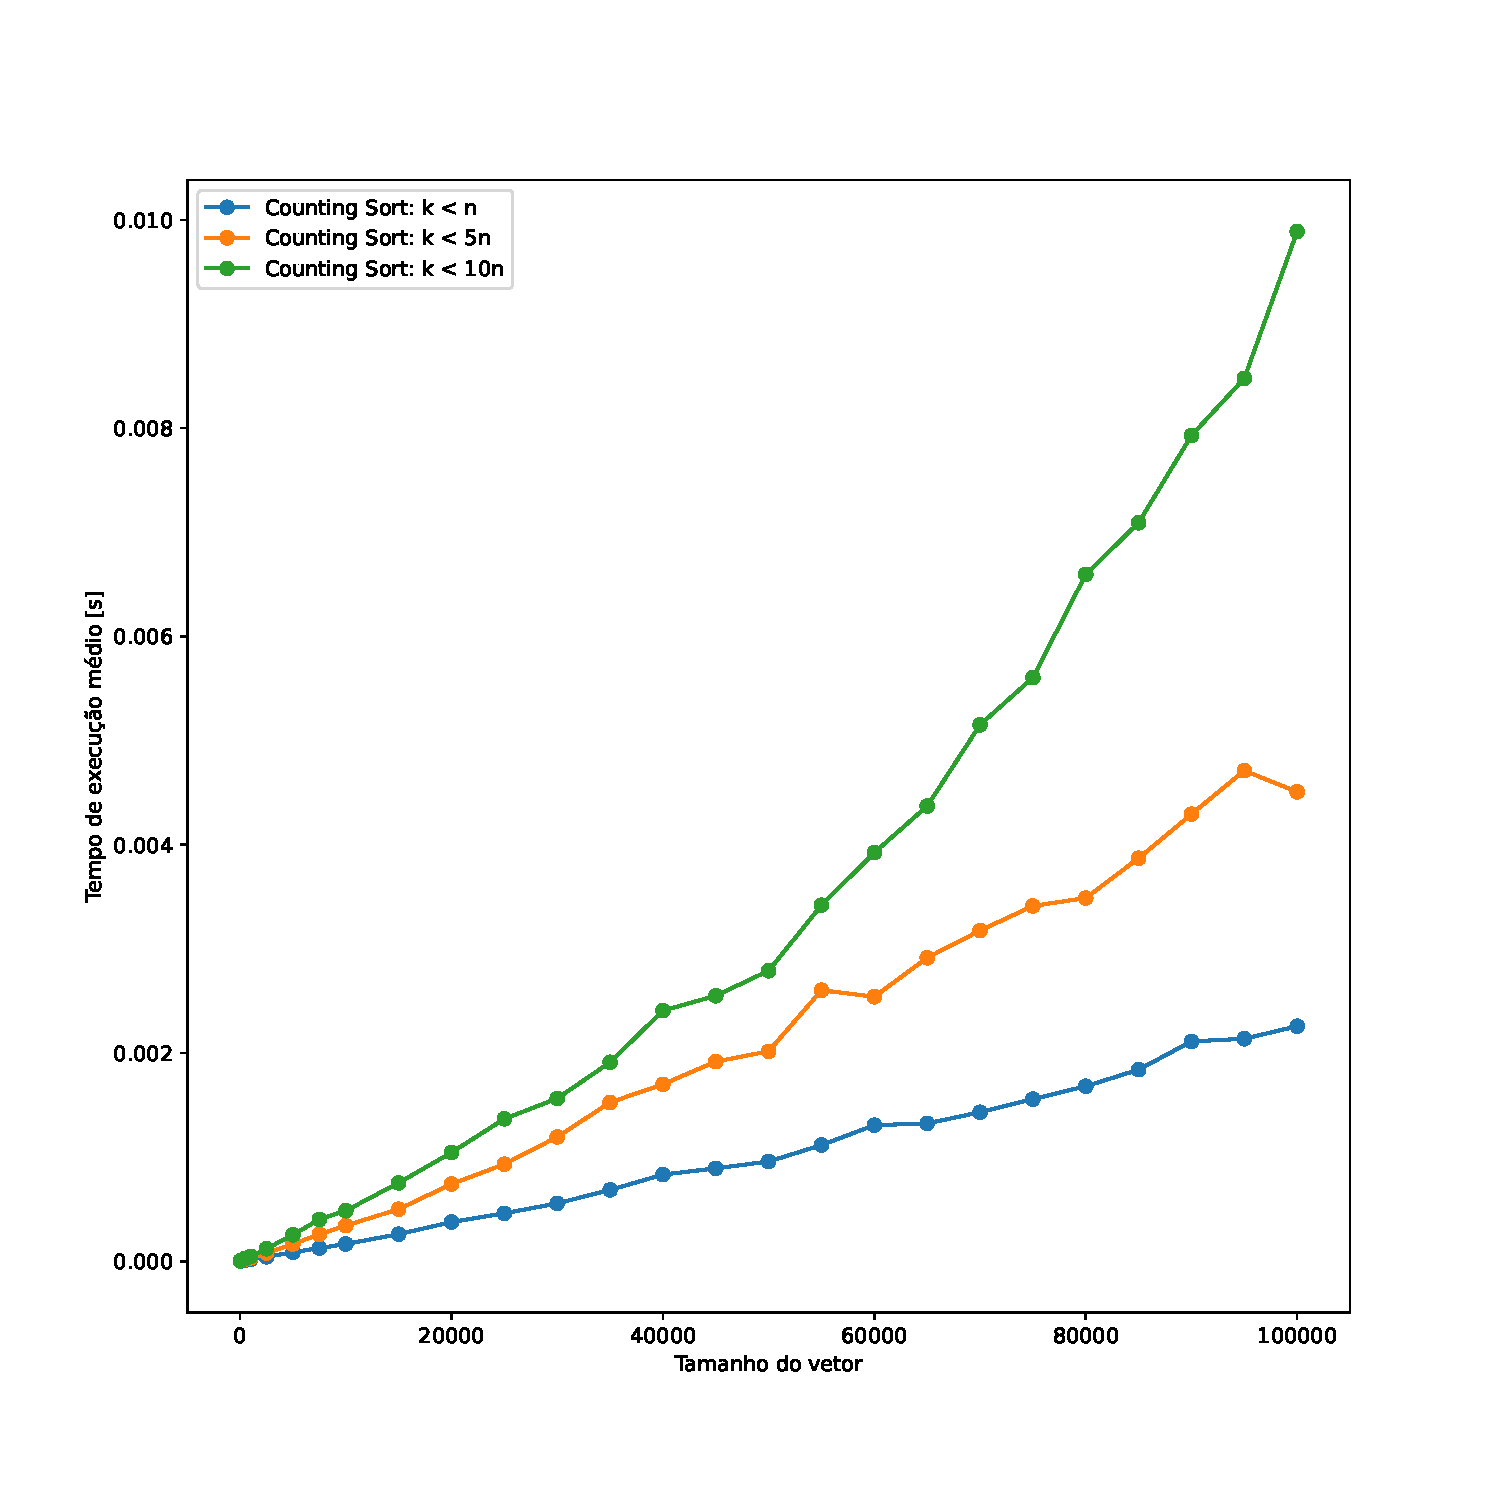
\includegraphics[scale=0.4]{imagens/counting.pdf}
    \caption{Resultado das medições temporais para o Counting Sort, ordenando valores com amplitude $k < n$, $k < 5n$ e $k < 10n$, respectivamente; a média de tempo de execução foi tirada a partir de 10 iterações para cada tamanho de vetor.}
    \label{Figura 4}
\end{center}
\end{figure}

\begin{figure}[H]
\begin{center}
    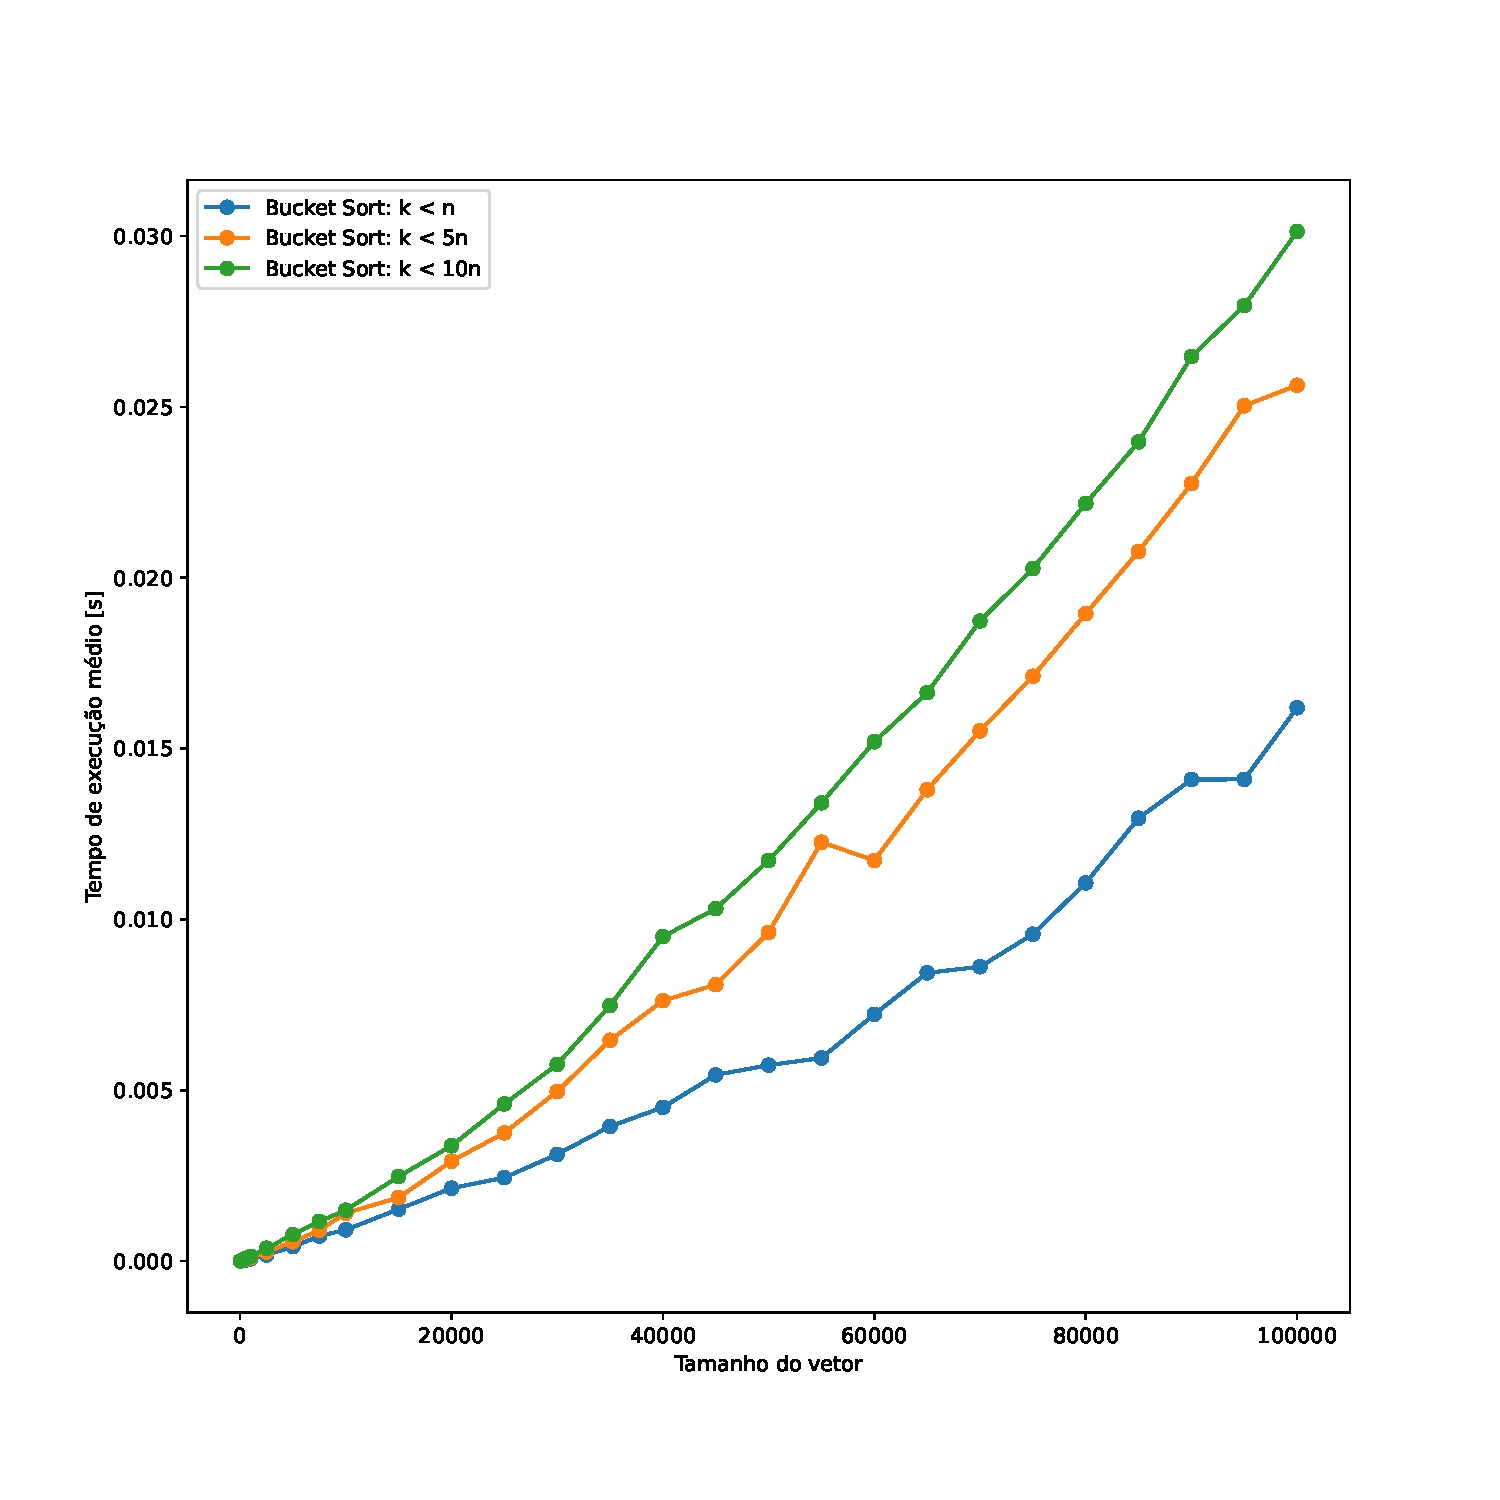
\includegraphics[scale=0.4]{imagens/bucket.pdf}
    \caption{Resultado das medições temporais para o Bucket Sort, ordenando valores com amplitude $k < n$, $k < 5n$ e $k < 10n$, respectivamente; a média de tempo de execução foi tirada a partir de 10 iterações para cada tamanho de vetor.}
    \label{Figura 5}
\end{center}
\end{figure}

\begin{figure}[H]
\begin{center}
    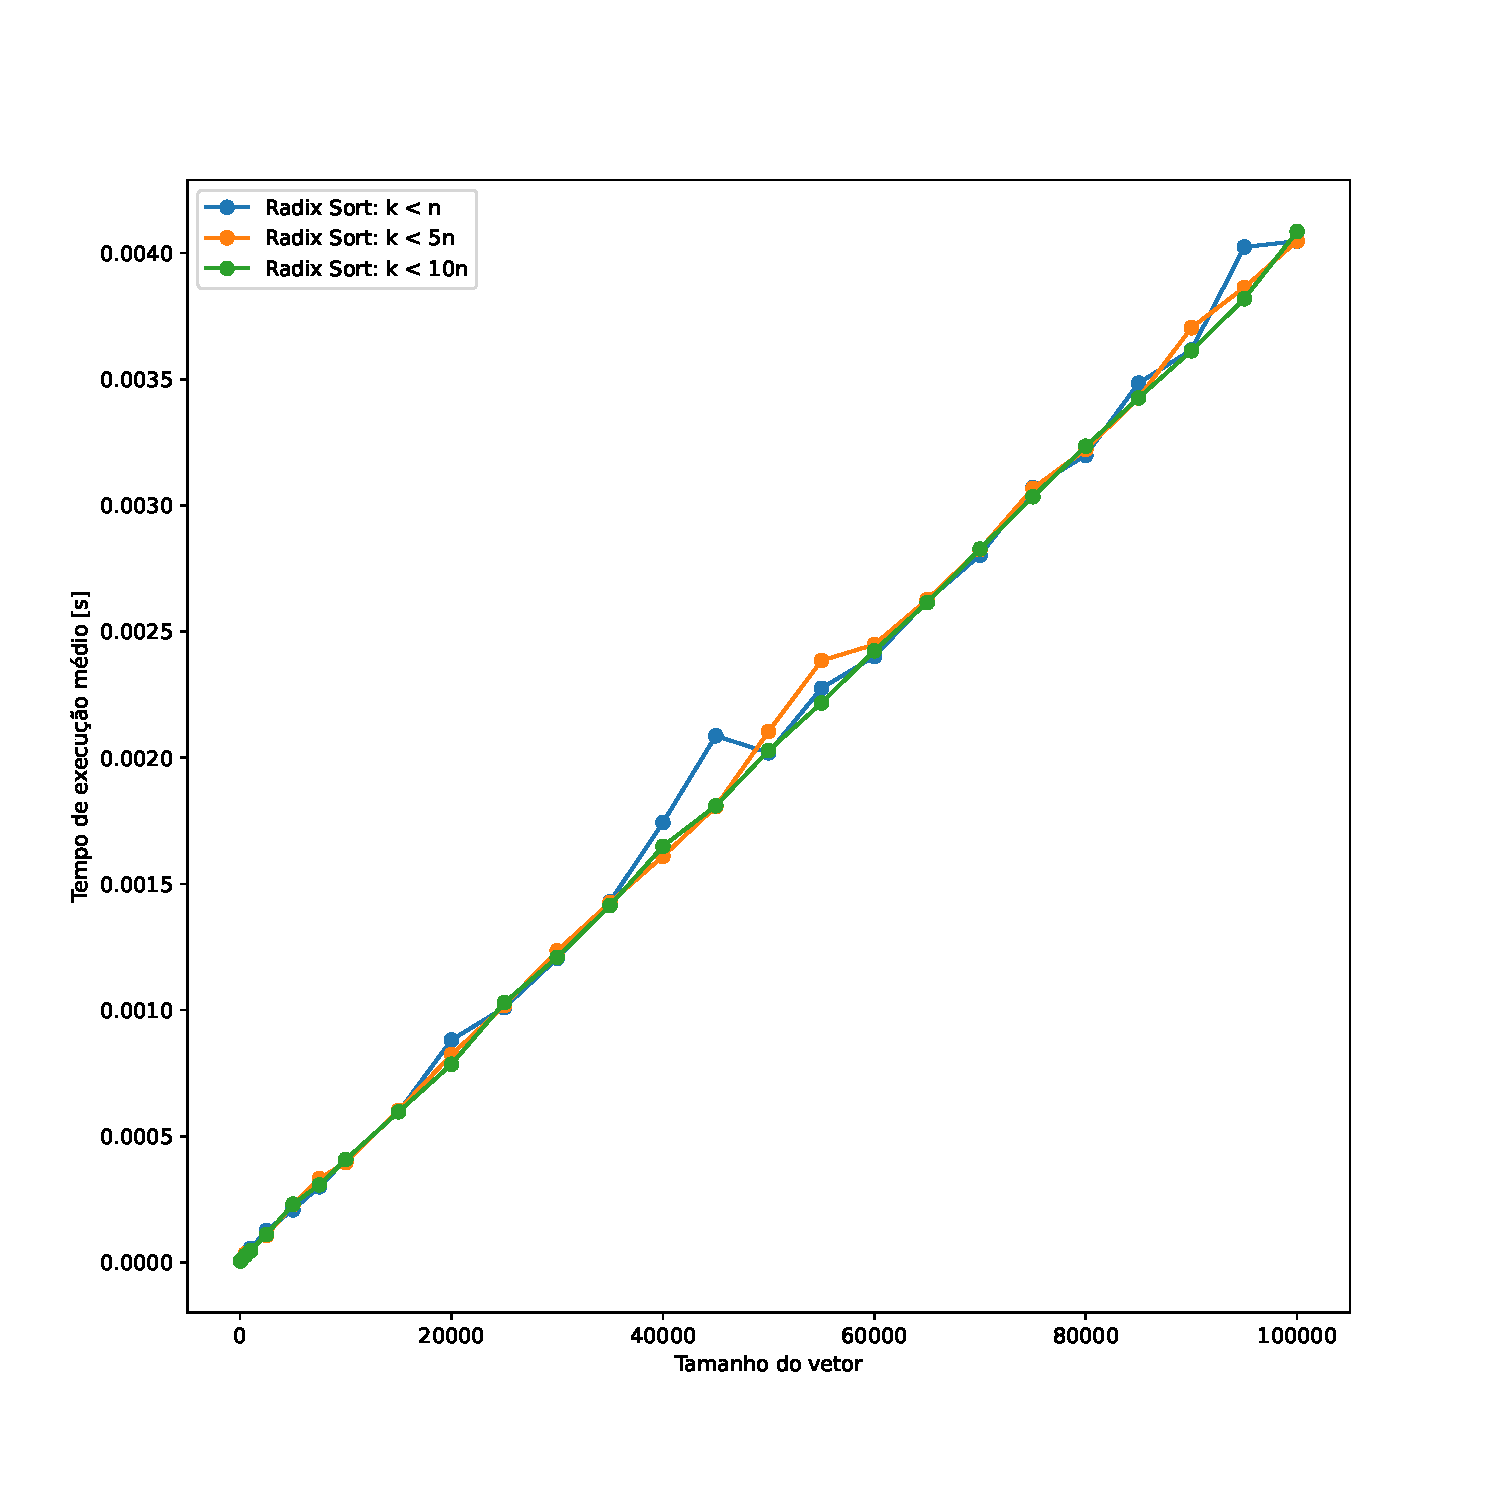
\includegraphics[scale=0.4]{imagens/radix.pdf}
    \caption{Resultado das medições temporais para o Radix Sort, ordenando valores com amplitude $k < n$, $k < 5n$ e $k < 10n$, respectivamente; a média de tempo de execução foi tirada a partir de 10 iterações para cada tamanho de vetor.}
    \label{Figura 6}
\end{center}
\end{figure}

\quad No gráfico da Figura 4, é possível observar que o desempenho do \textit{counting sort} de fato piora gradualmente com o aumento da amplitude das chaves; o mesmo ocorre com o \textit{bucketsort} (Figura 5). Já a eficiência do \textit{radix sort} (Figura 6) não foi afetada pelo aumento de $k$, visto que sua complexidade de tempo é $\mathcal{O}(d \cdot (n + b))$, ou seja, é afetada não por $k$, mas pela base e pelo número de dígitos das chaves, que permaneceram os mesmos.

%%%%% 3.2 COMPARAÇÃO %%%%%
\subsection{Comparação com Quick Sort, Heap Sort e Merge Sort}

\quad Por fim, o último experimento teve como objetivo comparar os métodos de ordenação lineares com o \textit{quicksort}, o \textit{heapsort} e o \textit{mergesort}, algoritmos de complexidade $\mathcal{O}(n \cdot log(n))$ estudados anteriormente\cite{relatorio1}\cite{relatorio2}. Foram realizados dois testes, com conjuntos de entrada cujas chaves foram geradas aleatoriamente respeitando diferentes amplitudes de valores ($k \leq 10.000$ e $k \leq 100.000$). Os outros critérios para cálculo do tempo médio de execução foram os mesmos adotados no experimento descrito no item 3.1 deste relatório.

\quad Na Figura 7, podemos observar que, para $k \leq 10.000$, os três métodos lineares mostraram-se mais rápidos que os de complexidade log-linear, como esperado. Quando elevamos a amplitude de valores entre as chaves para $k \leq 100.000$ (Figura 8), os algoritmos pertencentes a $\mathcal{O}(n \cdot log(n))$ mantiveram seu desempenho, enquanto o \textit{counting} e \textit{bucketsort} perderam vantagem; esta perda de vantagem foi pouco expressiva no caso do \textit{counting sort}, mas o \textit{bucketsort} mostrou-se, neste caso, também mais lento que o \textit{quicksort}.

\quad Na prática, o \textit{quicksort}, mesmo apresentando complexidade log-linear, ainda pode ser considerado muito rápido na ordenação de conjuntos de tamanhos $n \leq 100.000$, não ultrapassando o tempo médio de execução de 0,015 segundo.

\begin{figure}[]
\begin{center}
    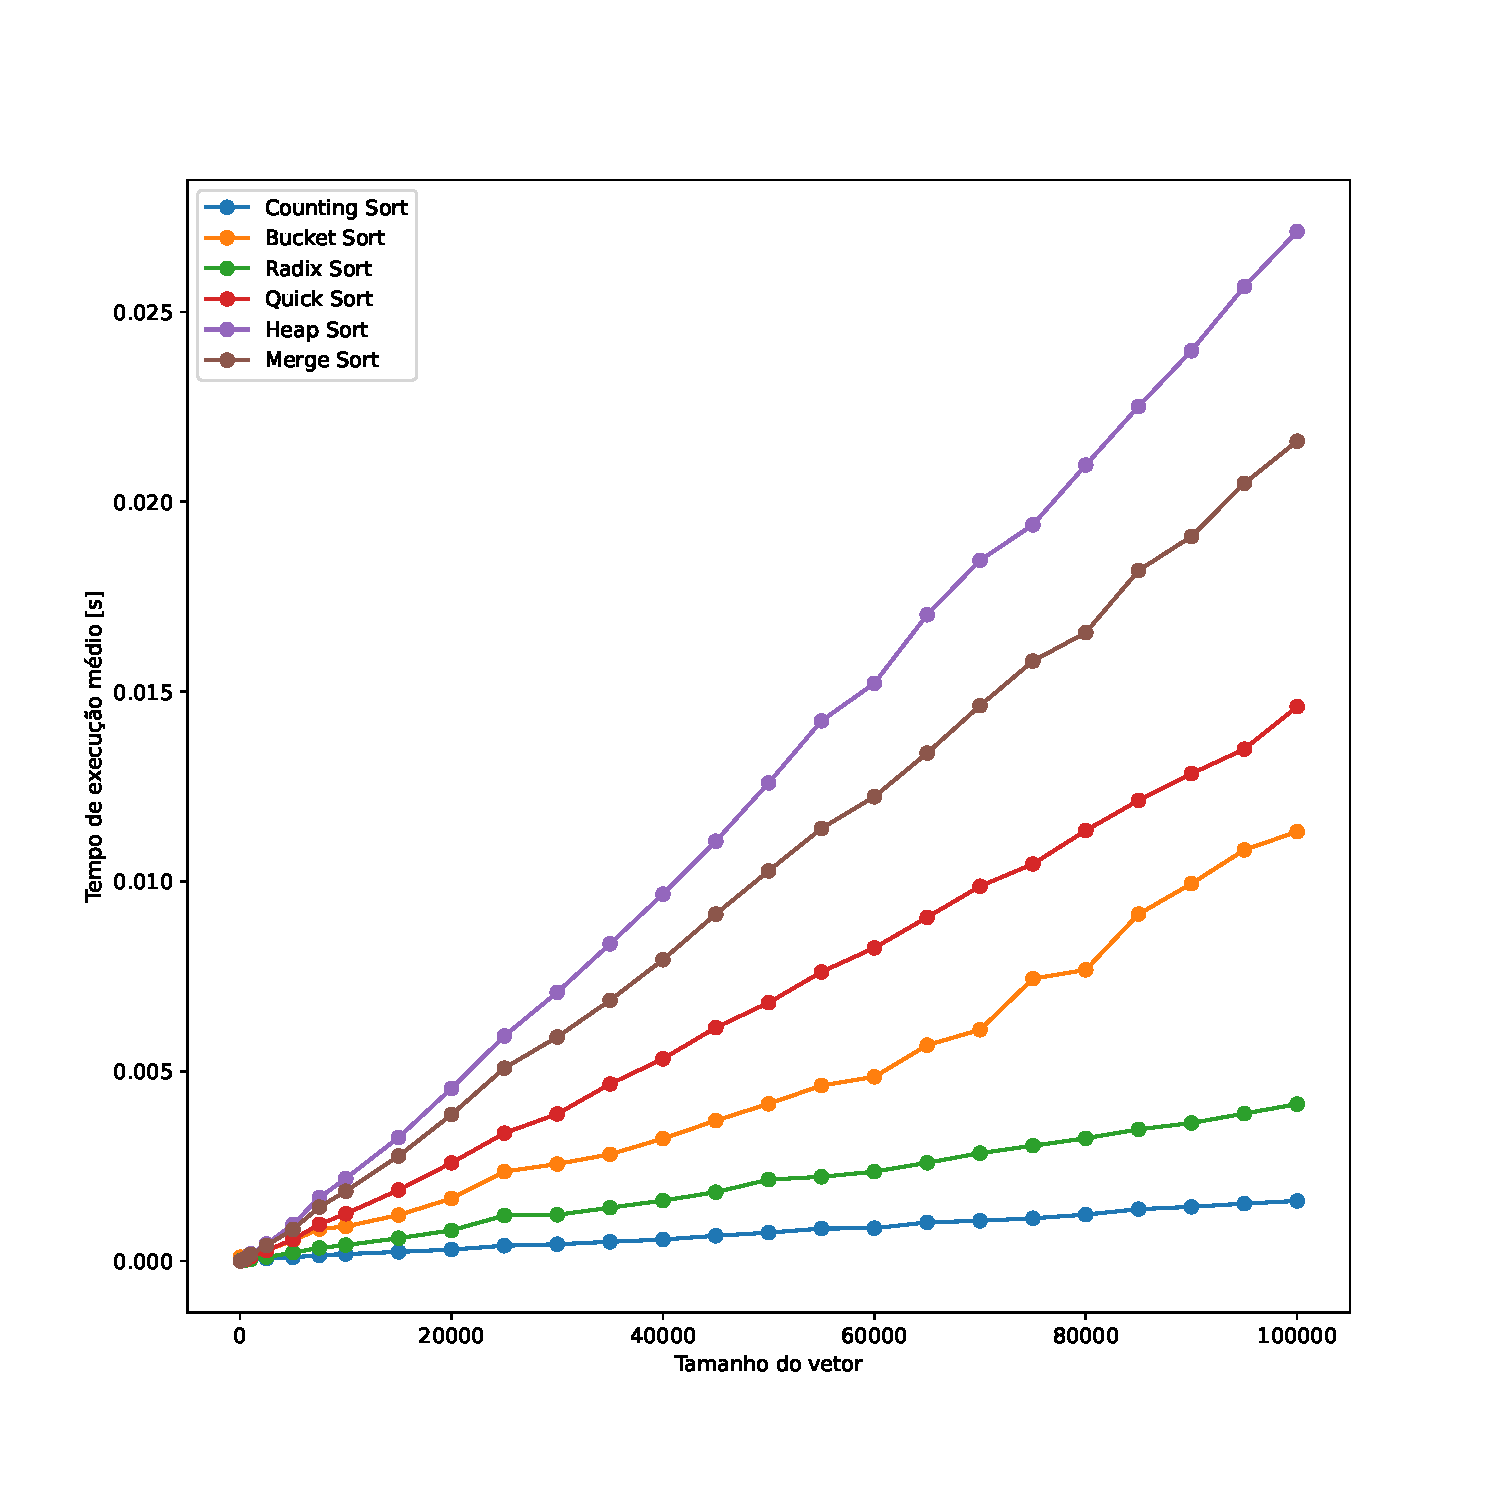
\includegraphics[scale=0.4]{imagens/0101.pdf}
    \caption{Resultado das medições temporais para cada algoritmo, ordenando com chaves de valores entre 0 e 10.000; a média de tempo de execução foi tirada a partir de 10 iterações para cada tamanho de vetor.}
    \label{Figura 7}
\end{center}
\end{figure}

\begin{figure}[]
\begin{center}
    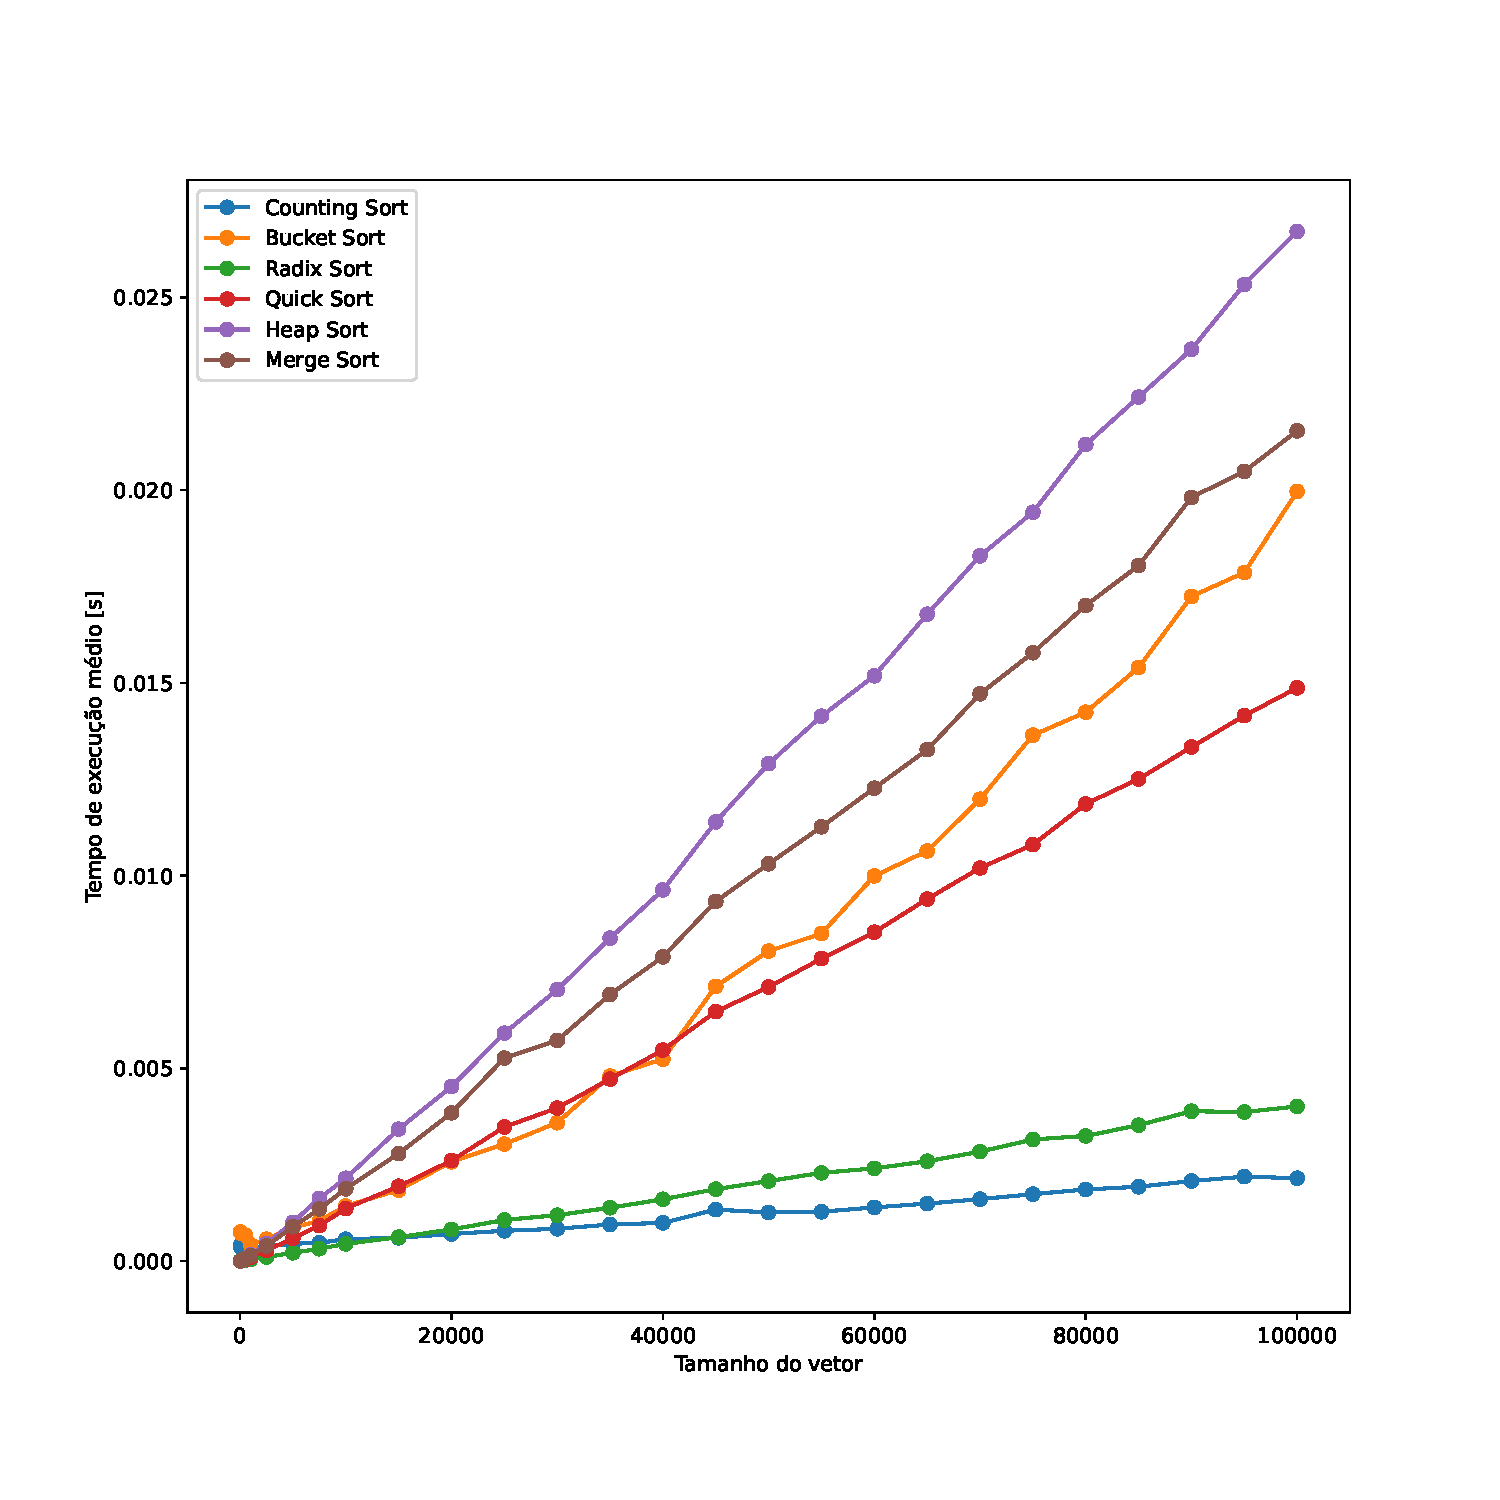
\includegraphics[scale=0.4]{imagens/0201.pdf}
    \caption{Resultado das medições temporais para cada algoritmo, ordenando com chaves de valores entre 0 e 100.000; a média de tempo de execução foi tirada a partir de 10 iterações para cada tamanho de vetor.}
    \label{Figura 8}
\end{center}
\end{figure}

\newpage
\quad Por fim, é preciso reforçar que, apesar de estes apresentarem menores tempos médios de execução, os algoritmos de ordenação lineares têm limitações, necessitando da alocação de memória auxiliar e não podendo trabalhar com chaves não inteiras. Para cenários em que a memória do sistema é escassa, ou quando os valores das chaves são reais, ainda é recomendado o uso de um algoritmo baseado em comparação, de complexidade log-linear.

\quad Ao escolher o melhor algoritmo para um dado problema, portanto, deve-se sempre levar em conta diversos fatores: o tamanho do conjunto a ser ordenado, a amplitude de valores das chaves nesse conjunto, a natureza de seus elementos e a memória disponível no sistema.

%%%%%%%%%%%%%%%%%%%%%%%%%%%%%%%%%%%%%%%%%%%%%%%%%%%%%%%%%%%
%%%                     4 CONCLUSÃO                     %%%
%%%%%%%%%%%%%%%%%%%%%%%%%%%%%%%%%%%%%%%%%%%%%%%%%%%%%%%%%%%
\section{Conclusão}
    %%%%%% Conclusão do relatório. O que você aprendeu nessa tarefa? %%%%%%
    
\quad Os métodos de ordenação lineares, para superarem a eficiência de $\mathcal{O}(n \cdot log(n))$, tem um custo adicional de alocação de memória auxiliar. Em suma, os algoritmos estudados apresentaram as seguintes características:

\begin{itemize}
    \item Para vetores de tamanho $n$ com amplitude de valores $k < 5n$, aproximadamente\footnote{Este foi o valor obtido experimentalmente.}, o \textit{counting sort} é o mais rápido dentre todos os algoritmos estudados. Quanto ao uso de memória, pertence a $\mathcal{O}(n + k)$.
    
    \item O \textit{radix sort} mostrou-se mais eficiente que o anterior quando a amplitude de valores $k$ ultrapassa $5n$, aproximadamente, sendo a melhor opção para cenários com chaves esparsas. Pode utilizar menos memória auxiliar que o \textit{counting} e o \textit{bucketsort}, pois, em sua sub-rotina, $k$ será sempre igual ao valor da base.
    
    \item Para a implementação utilizada, o \textit{bucketsort} é o mais lento dos três; no entanto, é um algoritmo versátil que pode ser otimizado e adaptado. Quanto ao uso de memória, também pertence a $\mathcal{O}(n + k)$.
\end{itemize}

\quad Sobre os algoritmos baseados em comparação — limitados inferiormente por $n \cdot log(n)$ — concluímos que ainda são a escolha recomendada para os cenários em que a memória do sistema é escassa, ou quando as chaves para ordenação não são discretas; dentre eles, o \textit{quicksort} possui o menor tempo médio de execução.

%%%%%%%%%%%%%%%%%%%%%%%%%%%%%%%%%%%%%%%%%%%%%%%%%%%%%%%%%%%
%%%                     REFERÊNCIAS                     %%%
%%%%%%%%%%%%%%%%%%%%%%%%%%%%%%%%%%%%%%%%%%%%%%%%%%%%%%%%%%%
\nocite{*}
\bibliographystyle{unsrt}
\bibliography{references.bib}
    %%%%%% Lembre-se de adicionar as referências bibliográficas utilizadas no arquivo 'references.bib'e depois cita-las nessa seção. Conulta: https://pt.overleaf.com/learn/latex/Bibliography_management_in_LaTeX %%%%%%

\end{document}